\documentclass{article}
\usepackage{svg}
\usepackage{array}
\usepackage{amsmath}
\usepackage{amsfonts} 
\usepackage{graphicx}
\usepackage{minted}
\usepackage[a4paper,  total={6.75in, 10in}]{geometry}
\usepackage[utf8]{inputenc}
\usepackage{hyperref}

\title{Animazione di una pandemia con un automa cellulare}
\author{Giulio Pastorello, Federico Gnudi}
\date{Novembre 2023}

\begin{document}

\maketitle

\section{Il Modello}

\hspace{\parindent}L'ispirazione principale per la seconda parte del progetto è 
stata il \textit{Game of Life} di Conway. Questo è il più famoso esempio di 
\textit{automa cellulare}: un insieme di celle posizionate in una griglia di forma 
predefinita, in cui lo stato di ogni cella varia all'avanzare del tempo e 
soddisfando alcune regole che dipendono dallo stato delle celle limitrofe. \\
Per simulare una pandemia  in una popolazione si è usato un modello simile a 
quello della prima parte. Le celle possono assumere quattro stati: 
\begin{itemize}
    \item S (sani)
    \item I (malati)
    \item R (guariti)
    \item Dead (morti)
\end{itemize}
Gli individui della popolazione possono evolvere solo in una precisa direzione: \\
\begin{figure}
    \centering
    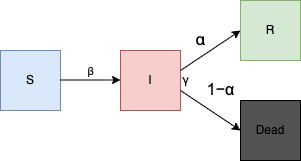
\includegraphics[width=0.4\paperwidth]{virus.drawio.png}
    \caption{\textit{Schema delle regole di evoluzione.}}
    \label{fig::virus}
\end{figure}
Un soggetto sano può contrarre il virus e diventare infetto, mentre un infetto
può sopravvivere alla malattia e guarire oppure morire. I passaggi di stato 
vengono regolati da parametri probabilistici che cercano di dare una simulazione
realistica della pandemia. \\
$\beta$ è il tasso di contagio che regola la probabilità di infezione; $\gamma$ è 
il tasso di rimozione per regolare la probabilità con la quale un infetto cambia 
stato da I a Dead o R; $\alpha$ dà la probabilità di morte una volta 
che l'individuo è stato rimosso, dunque $1-\alpha$ corrisponde alla probabilità di 
cura. \\
Il modello presenta similitudini con il Game of life, tuttavia presenta una 
sostanziale differenza: gli individui nel nostro modello saranno liberi di spostarsi 
lungo la griglia, mentre nel modello guida sono statici e cambiano il loro stato 
vivo/morto in base al numero di celle vicine vive e morte. 

\section{Il Codice}

\hspace{\parindent}Il programma presenta 2 file .cpp con relativi header files
(world.cpp e visual.cpp) e main.cpp come corpo principale. 
World.cpp definisce la griglia della simulazione attraverso la classe World e 
presenta tutti i metodi utili all'evoluzione del virus sulla popolazione infetta, 
mentre visual.cpp si occupa di visualizzare l'evoluzione del gioco a schermo 
attraverso l'utilizzo di librerie di SFML. \\
Entriamo ora più in dettaglio sulla classe World e sul file world.cpp. 

\begin{enumerate}
    \item \textbf{Definizione delle celle e metodo costruttore}\\
    \mint{C++}|enum class Cell {Dead, Empty, S, I, R };|
    Per definire lo stato delle celle abbiamo utilizzato un enum class Cell che 
    comprende tutti gli stati possibili delle celle. \\
    Le celle potranno quindi assumere 5 stati possibili. 4 di essi sono già stati 
    definiti nel modello, mentre lo stato Empty è necessario per permettere di avere 
    celle libere in cui gli individui possono spostarsi. \\
    La classe World presenta 2 attributi privati che sono \verb|m_side|, che 
    corrisponde alla dimensione del lato della griglia, e \verb|m_field| che 
    rappresenta la griglia in quanto vector di Cell. Il metodo costruttore \verb|World| 
    prende un intero a, che inizializza \verb|m_side|, e crea \verb|m_field| vettore 
    di Cell di dimensione $a*a$ con tutte celle Empty. 
    \mint{C++}|World::World(int a):m_side{a}, m_field(a*a, Cell::Empty){|
    \item \textbf{Metodi Get$\_$cell e Set$\_$cell}\\
    \begin{center}
    \begin{tabular}{ | m{4em} | m{4em} | m{4em} | m{4em} |}
        \hline 
        0 (0,0) & 1 (0,1) & 2 (0,2) & 3 (0,3) \\
        \hline
        4 (1,0) & 5 (1,1) & 6 (1,2) & 7 (1,3) \\
        \hline 
        8 (2,0) & 9 (2,1) & 10 (2,2) & 11 (2,3) \\
        \hline 
        12 (3,0) & 13 (3,1) & 14 (3,2) & 15 (3,3) \\
        \hline
    \end{tabular}
    \end{center}
    Oltre vari metodi per contare il numero di celle di un certo tipo e un metodo Get 
    per l'attributo privato \verb|m_side| la classe World presenta altri 2 metodi 
    interni: \verb|Get_cell| e \verb|Set_cell|. Tali metodi fungono da Get e Set per 
    gli elementi del vettore \verb|m_field| che corrisponde alla nostra griglia quadrata. 
    Siccome trattare gli elementi di una matrice quadrata con indici di un vettore 
    1-dimensionale era poco intuitivo abbiamo tradotto l'indice del singolo vettore 
    con $a*a$ elementi negli indici $(r, c)$ di una matrice quadrata di dimensione a.  
    Abbiamo adottato un ulteriore scelta di implementazione: la griglia quadrata è 
    toroidale. Dunque la griglia non ha bordi e vale il così detto “effetto Pacman”. 
    Questo è stato fatto per non incorrere in complicazioni dovute allo spostamento 
    di individui lungo i bordi, che avrebbero potuto volersi spostare in celle con 
    indice non valido.
    \mint{C++}|void Set_cell(Cell const& cell_type, int r, int c);|
    \mint{C++}|Cell Get_cell(int r, int c) const;|
    \item \textbf{Metodo initial$\_$random}\\
    \mint{C++}|void initial_random(World &world, int num_healthy, int num_infected)|
    Il metodo \verb|initial_random| genera casualmente nella griglia S e I 
    iniziali prendendo in ingresso un oggetto di tipo World e 2 interi. Questa 
    operazione viene realizzata attraverso cicli for in cui vengono generate casualmente 
    le posizioni degli individui che vanno posizionati. 
    Tale metodo presenta controlli sui parametri in ingresso per controllare che sia 
    presente almeno 1 infetto all'inizio e per evitare di inserire numeri non possibili. 
    Abbiamo tenuto la possibilità di riempire tutta la griglia poiché la simulazione 
    può avvenire anche se è un caso limite di poco interesse. 
    \item \textbf{Metodo infected$\_$counter} \\
    \mint{C++}|int infected_counter(World const &world, int r, int c);|
    Questo metodo si occupa semplicemente di contare il numero di infetti intorno ad 
    una determinata cella (r, c) e restituire tale numero. \\
    Tale metodo verrà ovviamente invocato solamente su celle sane poiché il numero di 
    malati vicini è un parametro che conta durante il contagio di un individuo. 
    \item \textbf{Metodi bool condition}\\
    Nel programma sono presenti diversi metodi bool. \\
    Il primo, \verb|move_condition|, prendendo in ingresso le coordinate (r, c) di una 
    cella restituisce vero se la cella non è morta e se ha una cella libera intorno a 
    sé in cui spostarsi. Questo metodo serve per distinguere il caso in cui l'individuo 
    è libero di spostarsi dal caso in cui invece è bloccato oppure è morto e quindi è 
    vincolato a rimanere dov'è. \\
    Sono inoltre presenti 3 metodi \verb|_condition| che si occupano di regolare i 
    passaggi fra gli stati delle celle. 
    \begin{itemize}
        \item \verb|infected_condition| prende in ingresso il numero di infetti vicini 
        e un parametro double $\beta$ per generare un numero intero casuale fra 0 e 100 
        e confrontarlo con il prodotto $20*\beta*\# infetti\, vicini$. Se il numero 
        casuale è minore del prodotto allora il metodo restituisce vero e la cella 
        sana per cui è stato chiamato chiamato verrà contagiata. 
        \item \verb|removal_condition| prende in ingresso un solo parametro double 
        $\gamma$ e analogamente al metodo precedente confronta un numero casuale fra 0 
        e 100 con il prodotto $100 *\gamma$. 
        Se il numero generato è minore del prodotto allora restituisce vero e quindi 
        l'infetto su cui è stato chiamato il metodo deve essere rimosso, ovvero 
        abbandona lo stato I per guarire o morire secondo quanto stabilito dal 
        prossimo metodo. 
        \item \verb|death_condition| è analogo al metodo prima, prende in ingresso un 
        parametro double $\alpha$. 
        Restituisce vero nel caso in cui il numero generato casualmente fra 0 e 100 
        è minore del prodotto $100 * \alpha$. Se restituisce vero l'individuo muore, 
        mentre se restituisce falso l'individuo sopravvive diventando R. 
        \item Come ultimo metodo bool troviamo \verb|virus_condition| che semplicemente 
        prende in ingresso un oggetto world e restituisce vero se il numero di I 
        è maggiore di zero. 
        Quest'ultimo metodo serve per capire se la pandemia può ancora svilupparsi. 
    \end{itemize}
    Come si può notare, attraverso la regolazione dei parametri in ingresso (compresi 
    fra 0 e 1) si può regolare quanto la malattia è contagiosa $(\beta)$, quanto il 
    virus dura in media $(\gamma)$ e quanto il virus sia letale $(\alpha)$. 
    \item \textbf{Metodo evolve}\\
    \mint{C++}|World evolve(World const &now,double beta, double gamma, double alpha){|
    Il metodo evolve è il fulcro del programma e si occupa di generare un nuovo oggetto 
    World a partire da uno di partenza in ingresso e dai parametri di probabilità 
    $\beta, \gamma, \alpha$.\\ 
    Questo metodo genera un copia del World attuale che verrà poi fatto evolvere e 
    comincia a scansionare le celle della griglia attuale. 
    Vengono distinti 2 casi con il metodo \verb|move_condition| che viene chiamato sul 
    mondo successivo poiché durante il ciclo di evoluzione la posizione delle celle 
    libere cambia e dunque deve seguire gli spostamenti aggiornati nel ciclo 
    continuamente.  \\
    Nel caso il metodo restituisca vero, la cella è viva e ha intorno almeno una casella 
    Empty, dunque viene spostata casualmente dove è libero ed evolve il suo stato a 
    seconda del suo stato attuale. Il tipo di evoluzione viene selezionata attraverso 
    uno switch case. \\
    Nel caso \verb|move_condition| sia falso invece si entra in una dinamica statica. 
    La cella è vincolata a rimanere nella sua posizione, tuttavia può comunque evolvere 
    il suo stato secondo le regole normali. 
    Ad ogni ciclo viene chiamato il Set sulla cella del mondo successivo per farla 
    cambiare e se si deve spostare viene chiamato il Set prima sulla cella di partenza,  
    che viene resa libera, e dopo sulla cella in cui arriva l'individuo. 
    Le celle Dead rientrano nel caso falso e rimarranno ferme durante tutta la pandemia.  
    \item \textbf{Metodi display}\\
    Sono presenti 2 ulteriori metodi che stampano a terminale il contenuto di una 
    griglia in 2 versioni diverse. Questi metodi sono stati utilizzati durante i test 
    e lo sviluppo del codice prima di introdurre la visualizzazione a schermo tramite 
    SFML. 
    Per completezza abbiamo deciso di tenerli. 
\end{enumerate}
Con questo si conclude la panoramica sul file world.cpp. 
Il file visual.cpp contiene una classe Visual in cui vengono utilizzate le librerie 
di SFML per ottenere 2 metodi in particolare che si occupano di disegnare la griglia 
\verb|(draw)| e di disegnare scritte \verb|(show_message)|. I metodi presentati vengono 
poi utilizzati nel main.cpp. 
\section{Compilazione}
\hspace{\parindent} Per costruire il programma si è deciso di usare 
\verb|cmake|, nel folder \verb|parte2/| è incluso il 
\verb|CMakeLists.txt| che permette di costruire il progetto 
(caricando la libreria SFML).\\
Per compilare serve fare la build con :
\begin{minted}{C++}
    cmake .  
    cmake --build .
\end{minted} 
Una volta fatto questo vengono prodotti due
eseguibili: \verb|virus_tty| e \verb|virus.test|. Oltre al file di test che viene
eseguito col CMake (\verb|virus.test.cpp|), viene consegnato anche un altro
file, \verb|virustest.cpp|, che era sstato usando nelle fasi preliminari del
progetto, prima di scrivere le funzioni che usano SFML. I test in questo file
non sono più utili per il funzionamento del programma ma vengono lasciati per 
completezza.
\subsection{Come compilare}
Per il progetto è necessario avere:
\begin{itemize}
    \item \verb|cmake| versione 16 o superiore;
    \item la libreria \verb|SFML|. Questa si scarica dal 
    \href{https://www.sfml-dev.org/}{suo sito}.
\end{itemize}
\section{Appendici}
\subsection{Git e Github}
Durante la realizzazione del progetto è stato fondamentale l'uso di 
Github per coordinare i lavori. Si lascia il 
\href{https://github.com/giuliopastorello/progetto_SMRV}{link} alla 
repository remota qualora potesse servire. Per usare il progetto senza
clonare la libreria di plotting si può semplicemente clonare la 
remote repository.
\subsection{Risorse}
\begin{itemize}
    \item cmake: \href{https://cmake.org/}{https://cmake.org/}
    \item SFML: \href{https://www.sfml-dev.org/}{https://www.sfml-dev.org/}
    \item github: \href{https://github.com/giuliopastorello/progetto_SMRV}{https://github.com/giuliopastorello/progettoSMRV}
\end{itemize}   
\end{document}